\subsubsection{Extension 4}
\begin{namedframe}{Cyclic quadrilaterals}
	\transglitter<2>[duration=5]
	\transcover<3>[duration=5]
	\begin{example}
		If $C_1$ and $C_2$ are two points on the circle, one on the minor arc $AB$ and the other on the major arc, prove that $\angle AC_1B + \angle AC_2B = \SI{180}{\degree}$.
		\vertspace
		This is equivalent to proving that the opposite angles of a cyclic quadrilateral are supplementary.
	\end{example}
	\centering
	\begin{tikzpicture}[scale=0.3]
		\coordinate [label=left:$O$](O) at (0,0);
		\coordinate [label=below left:$A$](A) at (-3,-4);
		\coordinate [label=right:$B$](B) at (4.75,-1.5612494996);
		\coordinate [label=below:$C_1$](C1) at (2,-4.58257569496);
		\coordinate [label=above:$C_2$](C2) at (-2,4.58257569496);

		\draw (O) circle (5);
		\draw (A) -- (C1) -- (B) -- (C2) -- cycle;
		\draw [dashed] (A) -- (O);
		\draw [dashed] (B) -- (O);
		\draw [dashed] (C1) -- (O);
		\draw [dashed] (C2) -- (O);

		\uncover<3->{\pic [draw, "$a$", angle eccentricity=1.5, angle radius=5mm] {angle = O--A--C2};}
		\uncover<3->{\pic [draw, "$a$", angle eccentricity=1.5, angle radius=5mm] {angle = A--C2--O};}

		\uncover<3->{\pic [draw, "$b$", angle eccentricity=1.5, angle radius=6mm] {angle = C2--B--O};}
		\uncover<3->{\pic [draw, "$b$", angle eccentricity=1.5, angle radius=6mm] {angle = O--C2--B};}

		\uncover<3->{\pic [draw, "$c$", angle eccentricity=1.5, angle radius=3mm] {angle = O--B--C1};}
		\uncover<3->{\pic [draw, "$c$", angle eccentricity=1.5, angle radius=3mm] {angle = B--C1--O};}

		\uncover<3->{\pic [draw, "$d$", angle eccentricity=1.5, angle radius=4mm] {angle = C1--A--O};}
		\uncover<3->{\pic [draw, "$d$", angle eccentricity=1.5, angle radius=4mm] {angle = O--C1--A};}
	\end{tikzpicture}
	\hspace{1cm}
	\uncover<2-2>{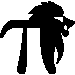
\includegraphics[height=20ex]{../Logo}}
\end{namedframe}
\begin{namedframe}{Extension 4 proof}
	\begin{proof}[Proof that opposite angles of a cycle quadrilateral are supplementary.]
		\begin{wrapfigure}{l}{0pt}
			\begin{tikzpicture}[scale=0.3]
				\coordinate [label=left:$O$](O) at (0,0);
				\coordinate [label=below left:$A$](A) at (-3,-4);
				\coordinate [label=right:$B$](B) at (4.75,-1.5612494996);
				\coordinate [label=below:$C_1$](C1) at (2,-4.58257569496);
				\coordinate [label=above:$C_2$](C2) at (-2,4.58257569496);

				\draw (O) circle (5);
				\draw (A) -- (C1) -- (B) -- (C2) -- cycle;
				\draw [dashed] (A) -- (O);
				\draw [dashed] (B) -- (O);
				\draw [dashed] (C1) -- (O);
				\draw [dashed] (C2) -- (O);

				\pic [draw, "$a$", angle eccentricity=1.5, angle radius=5mm] {angle = O--A--C2};
				\pic [draw, "$a$", angle eccentricity=1.5, angle radius=5mm] {angle = A--C2--O};

				\pic [draw, "$b$", angle eccentricity=1.5, angle radius=6mm] {angle = C2--B--O};
				\pic [draw, "$b$", angle eccentricity=1.5, angle radius=6mm] {angle = O--C2--B};

				\pic [draw, "$c$", angle eccentricity=1.5, angle radius=3mm] {angle = O--B--C1};
				\pic [draw, "$c$", angle eccentricity=1.5, angle radius=3mm] {angle = B--C1--O};

				\pic [draw, "$d$", angle eccentricity=1.5, angle radius=4mm] {angle = C1--A--O};
				\pic [draw, "$d$", angle eccentricity=1.5, angle radius=4mm] {angle = O--C1--A};
			\end{tikzpicture}
		\end{wrapfigure}
		\pause
		The sum of the interior angles of a quadrilateral equals \pause $\SI{360}{\degree}$.
		\sep
		So:
		\begin{align*}
			\uncover<+->{a + b + c + d + a + b + c + d &= \SI{360}{\degree}\\}
			\uncover<+->{2(a + b + c + d) &= \SI{360}{\degree}\\}
			\uncover<+->{a + b + c + d &= \SI{180}{\degree}}
		\end{align*}
		\uncover<6->{\qedhere}
	\end{proof}
\end{namedframe}
